\documentclass{article}
\usepackage{amsmath}
\usepackage{amssymb}
\usepackage{graphicx}
\title{Predicting Wall Conditioning}
\author{Arthur Adriaens}

\begin{document}
\maketitle
\section*{\textit{Theory}}
When a material has been subjected to impurities, these impurities will be
stored in interstitial lattice sites  (LS). The base material atoms are bound
by a certain energy $E_b$ whilst the trapped impurity is bound by $E_t$, as
most often $\mid E_t\mid <\mid E_b\mid $, wall conditioning in fusion reactors is effective.  
In general GDC (glow discharge wall conditioning) creates low energy ions
which propagate to the wall as no magnetic field is present. Ion cyclotron 
wall conditioning creates low-energy charge exchange neutrals (i.e
neutrals who have gained their energy through charge exchange) who, as they are
not confined, move towards the wall. Ideally these ions and neutrals have energies
sufficient to de-trap (sputter) the impurities but are still below the energy
necessary to sputter the base material.  Mathematically we can express the
amount of impurities leaving the wall per area ($m^2$) as a functional of the form:
\begin{equation}
    \mathcal{I}[n] = \sum_j\int_E \int_\theta Y_{jI}(n(t,\mathbf{r}),E,\theta)\mathfrak{F}_j(E,\theta)
\end{equation}
Whereby $Y_{Ij}(n(t,\mathbf{r}),E,\theta)$ is the impurity concentration-, energy- and
angle of incidence-dependent impurity sputtering rate (i.e \#out/\#in) for
incoming species j and $\mathfrak{F}_j(E,\theta)$ is the incoming particle
distribution ($\frac{\text{particles}}{m^2s}$) for species j.  The base
material sputtering rate may be given by:
\begin{equation}
    B = \sum_j\int_\theta \int_E Y_{jB}(E,\theta)\mathfrak{F}_j(E,\theta)
\end{equation}
In full, the total amount of particles leaving the wall per second per unit area
is thus:
\begin{equation}
    W(t) \stackrel{\Delta}{=} \mathcal{I}[n] + B = \sum_j \int_\theta \int_E \left\{ Y_{jI}(n(t,\mathbf{r}),E,\theta) + Y_{jB}(E,\theta) \right\} \mathfrak{F}_j(E,\theta)
\end{equation}
\newpage
\section*{\textit{Simulation: homogeneous doping and erosion}} 
To simulate $Y_{jI}$ it is necessary to create a model, the chosen model is 1D
and consists of a slab of the base material with a certain concentration of
$E_t$ bound impurities. As we will be using the BCA, more specifically
rustBCA\cite{rustBCA}, our simulations are dependent on how we choose our
parameters, namely the cutoff energy $E_c$, the displacement energy $E_d$ , the
bulk binding energy $E_b$ and the surface binding energy $E_s$ \cite{Eckstein}.
As we're dealing with sputtering, we will ignore $E_d$ and take $E_c$ to be
small enough (e.g 1\% of the input energy). In most codes $E_b$ is taken to be
0 and only $E_s$ is varied, we will not proceed this way as this omits some
physics, we will take $E_b$ to be a reported value for the base material and
$E_s = \Delta H_s - E_b$, i.e the heat sublimation is the energy to dislodge an
atom from the lattice and transport it to outside the material. As a lot of current
research on wall conditioning concerns boron on tungsten or graphite
substrates, with boron having a measured density of $1.1$ g/cm$^3$ on TOMAS, we will
focus on boron of number density
\begin{equation}
    \frac{1.1}{10.81}\times \frac{N_a}{10^{24}} = 0.06128 \frac{\text{atoms}}{\text{\AA}^3}
\end{equation}
Note that $1.1$ g/cm$^3$ is considerable lower than in most of the literature, we assume
that this is inherent to the method of layer growth used, namely magnetron sputtering.
For pure boron $\Delta H_s=5.6$eV \cite{BoronSubl} and as usually $E_s = 5.73$ is taken,
we will take $E_b = 0.13$eV.
For the impurities we will assume they have both $E_s$ and $E_b$ equal zero.
The simplest model considers the impurities
to be homogeneously distributed in the slab and to erode homogeneously.
Simple BCA simulations using these parameters for different angles shows the following behaviour (20\% impurity doping):
\begin{figure}[ht]
    \centering
    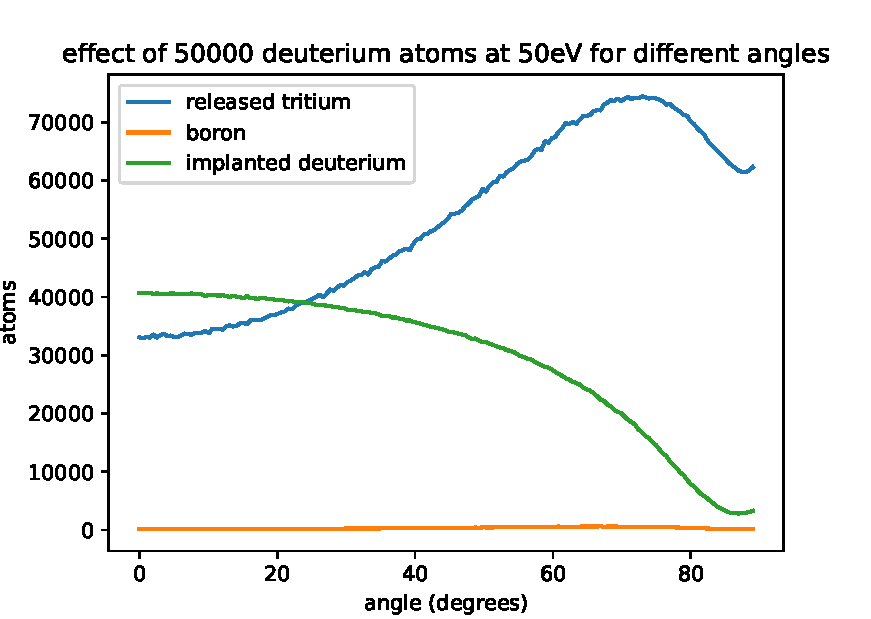
\includegraphics[width=0.7\textwidth]{figures/detrapex.pdf}
\end{figure}\\
Although this yields insight in how angle dependence plays a role, it is not in general easily measurable.
A quantity that is in general measured is the outgassing in function of time, as such we need to add time-dependence
to our model.
The amount of impurities in a slab of area A and depth D prior to any 
wall conditioning may be given by
$N_0 = n_0\times A \times D$, after one timestep $\Delta t$ the amount will have been reduced
by $\sum_jY_{jI}(n(t),E,\theta)\mathfrak{F}_j(E,\theta)\times A\times\Delta t\stackrel{\Delta}{=}\mathcal{I}[n(t)]A\Delta t $ .
The amount of impurities in the material thus follows (if we assume homogeneous erosion):
\begin{equation}
    \frac{\text{d}N(t)}{\text{d}t} = AD\frac{\text{d}n(t)}{\text{d}t} = -A\mathcal{I}[n(t)]
\end{equation}
We thus have that the concentration of impurities in the slab changes as 
\begin{equation}
    \frac{\text{d} n}{\text{d} t} = -\frac{\bar{\mathcal{I}}[n(t)]}{D}
\end{equation}
We need to solve this equation to determine the amount of impurities sputtered per second per unit area
$\bar{\mathcal{I}}[n(t)]$, e.g forward euler we would start from a certain $n = n_0$ and change n according
to
\begin{equation}
    \Delta n = -\frac{\bar{\mathcal{I}}[n(t)]}{D}\Delta t
\end{equation}
We will start with GD in H$_2$ of which we have ion energy distributions from an RFEA:
\begin{figure}[ht]
    \centering
    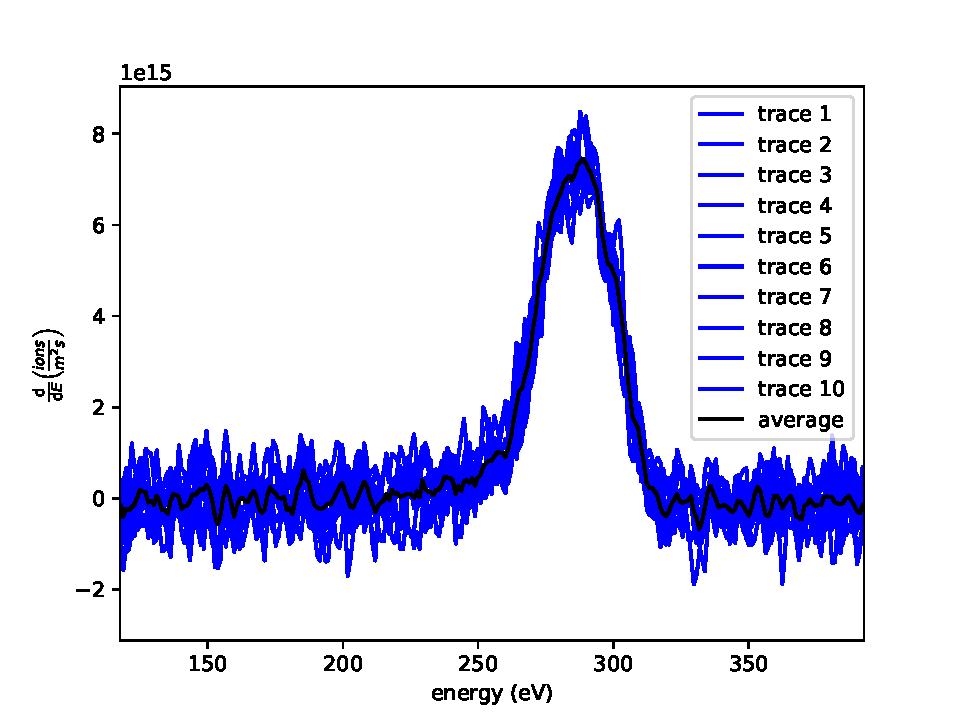
\includegraphics[width=0.8\textwidth]{figures/RFEAex.pdf}
\end{figure}\\
Here obviously $\bar{\mathfrak{F}}_j(E,\theta) \stackrel{\Delta}{=} \frac{\mathfrak{F}_j(E,\theta)}{\Delta E}$ is the y-axis,
we also assume equal angle likeliness, as such:
\begin{equation}
    \mathcal{I}[n] = \frac{1}{N}\sum_j\sum_E \sum_\theta^N Y_{jI}(n(t,\mathbf{r}),E,\theta)\bar{\mathfrak{F}}_j(E,\theta)\Delta E
\end{equation}
Where we kept the summation over $j$ as multiple species may be present which may be accounted for (not only H$^+$
but also H$_2^+$, H, H$_3^+$,...)
%\section*{\textit{temp}}
%As is well known, when a material is subjected to a plasma a sheath forms
%abiding by Poisson's equation
%\begin{equation}
%    \chi^{\prime\prime} = \left( 1 + \frac{2\chi}{\mathfrak{M}^2}\right)^{-\frac{1}{2}} - e^{-\chi}
%\end{equation}
%with 
%\begin{equation*}
%    \chi \stackrel{\Delta}{=} - \frac{e\phi}{KTe} \qquad \epsilon \stackrel{\Delta}{=} \frac{x}{\lambda_D} = x\left(\frac{n_0e^2}{\epsilon_0 KT_e}\right)^{1/2} \qquad \mathfrak{M} \stackrel{\Delta}{=} \frac{u_0}{(KTe/M)^{1/2}}
%\end{equation*}
\section*{\textit{Compare with experiments}}
$\mathfrak{F}_j(E) \stackrel{\Delta}{=} \int_\theta \mathfrak{F}_j(E,\theta)$ is
a measureable quantity, for example on TOMAS the neutral fluxes are measureable
\cite{DanielNPA} as well as the ions \cite{AndreiRFEA}. As such, an angle distribution needs
to be chosen, e.g 
\begin{equation}
    \tilde{\mathfrak{F}}_j(E,\theta) \stackrel{\Delta}{=} \frac{2cos^2(\theta)}{\pi}\mathfrak{F}_j(E)
\end{equation}
$Y_{jB}$ on it's own is straightforward to simulate using e.g rustBCA using known material
parameters, the difficulty lies in simulating the compound, and thus devising $Y_{jI}$.

\bibliographystyle{plain}
\bibliography{sources}
\end{document}
